\documentclass{beamer}
\usetheme{Boadilla}
\usepackage{tikz}
\usepackage{listings}
\usepackage{hyperref}
\begin{document}
\title{Sentiment analysis using live Twitter streaming API and Python}
\subtitle{Course: AE-663,Group: P13}
\author{Monika Sahai:
\texttt{133079022}
\and
Zeal Sheth:
\texttt{133079023}
}
\institute{Indian Institute Of Technology, Bombay}
\date{\today}

\begin{frame}
\titlepage
\end{frame}

\begin{frame}
\frametitle{Outline}
\tableofcontents
\end{frame}

\section{Introduction}

\subsection{Sentiment analysis}
\begin{frame}
\frametitle{Sentiment Analysis}
\begin{enumerate}
\item What is sentiment analysis?\\
Process of identifying and characterizing the opinions expressed in a text to determine if the writer's emotion is positive,negative or neutral.\\
\item Why is it useful?
\begin{enumerate}
\item Companies use sentiment analysis to improve their business.\\
Ex: Customer responses(feedback forms) can be analyzed to calculate the customer satisfaction index.
\item Powerful method for analysis of business in share market.
\end{enumerate}
\end{enumerate}
\end{frame}



\subsection{Twitter API}
\begin{frame}
\frametitle{Twitter API}
\begin{enumerate}
\item Steps to connect to API
\begin{enumerate}[I]
\item Create a twitter account.
\item Go to https://apps.twitter.com/ and log in with your twitter credentials.
\item Click "Create New App"
\item Fill out the form, agree to the terms, and click "Create your Twitter application"
\item In the next page, click on "API keys" tab, and copy your "API key" and "API secret".
\item Scroll down and click "Create my access token", and copy your "Access token" and "Access token secret".
\end{enumerate}
\item These keys and tokens are used for connecting to twitter and streaming live tweets.
\item API returns the result in json format
\end{enumerate}
\end{frame}

\begin{frame}
\frametitle{Twitter API}
\begin{enumerate}
\item Rest and Streaming API 
\begin{enumerate}       
\item Search/REST API
\begin{itemize}
\item Search goes back in time (up to a week) to find tweets that have already been sent.
\item  HTTP stream is not continous.
\end{itemize}

\item Streaming API
\begin{itemize}
\item Stream goes forward in time (starting from when you initiate the call) to capture new tweets in (more or less) real time as they are sent.        
\item Requires keeping a persistent HTTP connection open. 
\end{itemize}
\end{enumerate}
\end{enumerate}
\end{frame}


\subsection{REST vs Streaming API}
\begin{frame}
\frametitle{REST vs Streaming API}
\begin{columns}[t]
\column{0.5\textwidth}
\begin{figure}
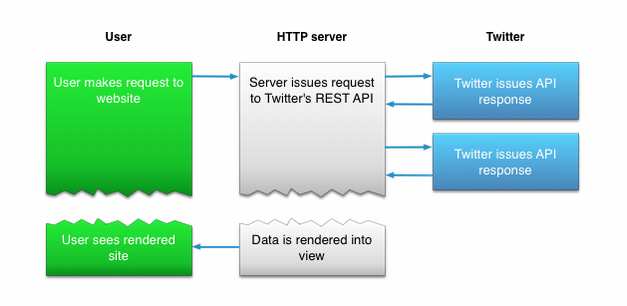
\includegraphics[width=7cm,height=4.1cm]{./Images/REST_API.png}
\caption{REST API}
\end{figure}
\column{0.5\textwidth}
\begin{figure}
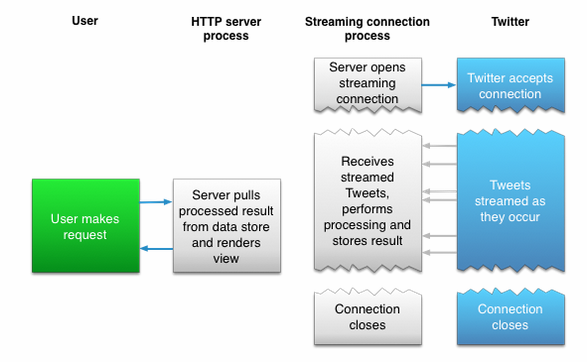
\includegraphics[width=6cm,height=4.5cm]{./Images/Streaming_API.png}
\caption{Streaming API}
\end{figure}
\end{columns}
\end{frame}

\section{Packages used}
\begin{frame}
\frametitle{Packages used}
\begin{enumerate}
\item nltk : used for data mining
\item re : used for filtering tweets
\item tweepy : Python library for twitter API
\item json : for reading the data collected by twitter streaming.
\item matplotlib : Package for visualizing the data in graphical form.
\item Matplotlib Basemap toolkit : Library for geo-plotting
\end{enumerate}
\end{frame}


\subsection{NLTK}
\begin{frame}
\frametitle{NLTK}
\begin{enumerate}
\item NLTK: Natural Language Processing Toolkit
\item Phases of classifier:
\begin{enumerate}
\item Phase-I : Training of the classifier
\item Phase-II : Testing of the classifier
\end{enumerate}

\item We have used a database of 2500 tweets as sample data whose sentiments are known.
\item This data is used to extract features for sentiment analysis.
\item Feature list is then given to classifier for training.
\item Testing of the classifier is done by calling the trained classifier on data to be analysed i.e. tweets.
\end{enumerate}
\end{frame}


\begin{frame}
\frametitle{Sentiment analysis flow}
\begin{figure}
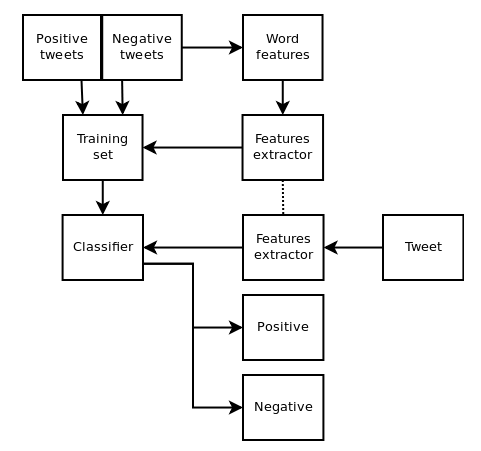
\includegraphics[scale=0.45]{./Images/NLTK.png}
\caption{Training and Testing of Bayes classifier}
\end{figure}
\end{frame}
\subsection{Tweepy}
\begin{frame}
\frametitle{Tweepy}
\begin{enumerate}
\item Provides Classes and methods for connecting to API and streaming namely
OAuthHandler\\
\begin{figure}

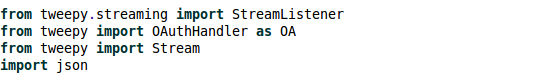
\includegraphics[width=9cm,height=1cm]{./Images/Import.png}
\end{figure}

\begin{figure}
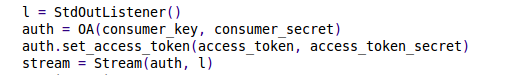
\includegraphics[width=8cm,height=1cm]{./Images/OAuth.png}
\caption{Usage of OAuthHandler}
\end{figure}
\end{enumerate}
\end{frame}





\subsection{Matplotlib}


\begin{frame}
\frametitle{Matplotlib}

\begin{enumerate}
\item Basemap
\begin{enumerate}
\item[]
\begin{figure}

\includegraphics[scale=0.3]{./Images/BaseMap}
\caption{Setting the basemap}
\end{figure}

\item provides the facilities to transform coordinates to one of 25 different map projections.
\end{enumerate}

\item Shapefiles:
\begin{enumerate}
\item  Contains geographical data.
\item It is developed and regulated by Esri ( Environmental Systems Research Institute)
\item The shapefile format is a digital vector storage format for storing geometric location and associated attribute information.
\end{enumerate}
\end{enumerate}
\end{frame}

\begin{frame}

\frametitle{Matplotlib contd.}
\begin{enumerate}
\item Matplotlib is then used to plot the points in the transformed coordinates.
\begin{enumerate}
\item Shape file is read and polygons are constructed using the parameters obtained from the shape file.
\item Polygon library is used to generate polygon from shapefiles.
\item Used modules colors and patches to fill the polygons states on map with different colors.
\end{enumerate}  
\end{enumerate} 
\end{frame}

\section{Control flow}
\begin{frame}
\frametitle{Control Flow}
\begin{enumerate}
\item Streaming
\item Feature extraction
\item Sentiment categorization as positive,negative or neutral
\item Constructing polygons for states using shapefile
\item Assigning colors to polygons based on the happiness score
\item Plotting the map with set properties
\end{enumerate}
\end{frame}


\section{Results}
\subsection{Time wise sentiment graph}
\begin{frame}
\frametitle{Happiness score distribution}
\begin{columns}
\column{0.5\textwidth}
\begin{figure}
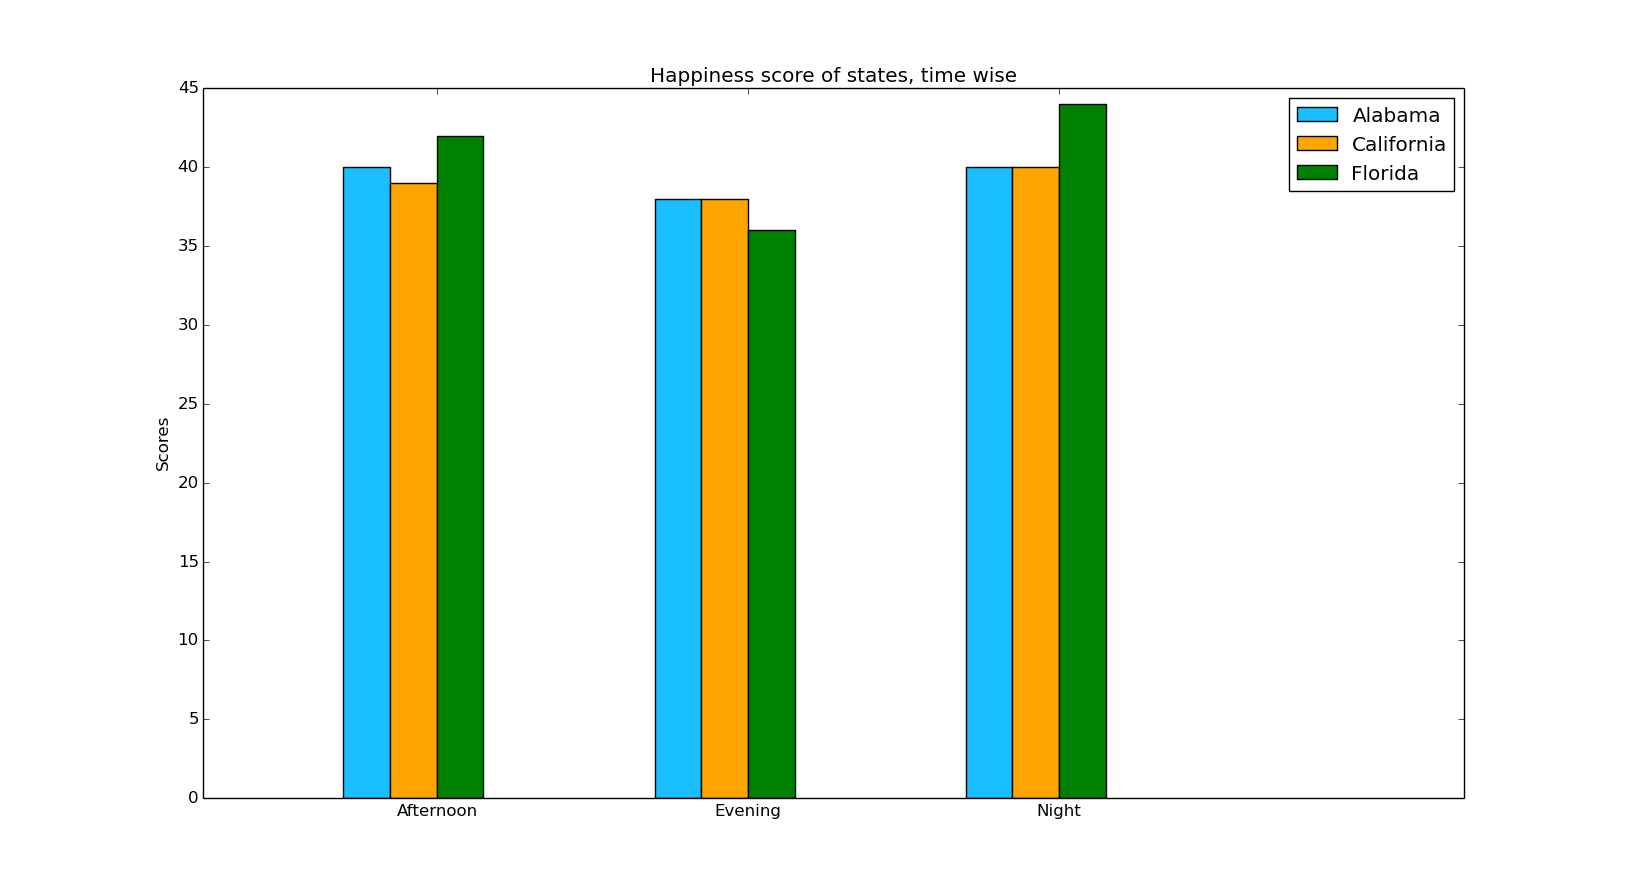
\includegraphics[scale=0.15]{./Images/Time_in_day50}
\caption{Happiness score for different times of the day for sample of 50 tweets}
\end{figure}

\column{0.5\textwidth}
\begin{figure}
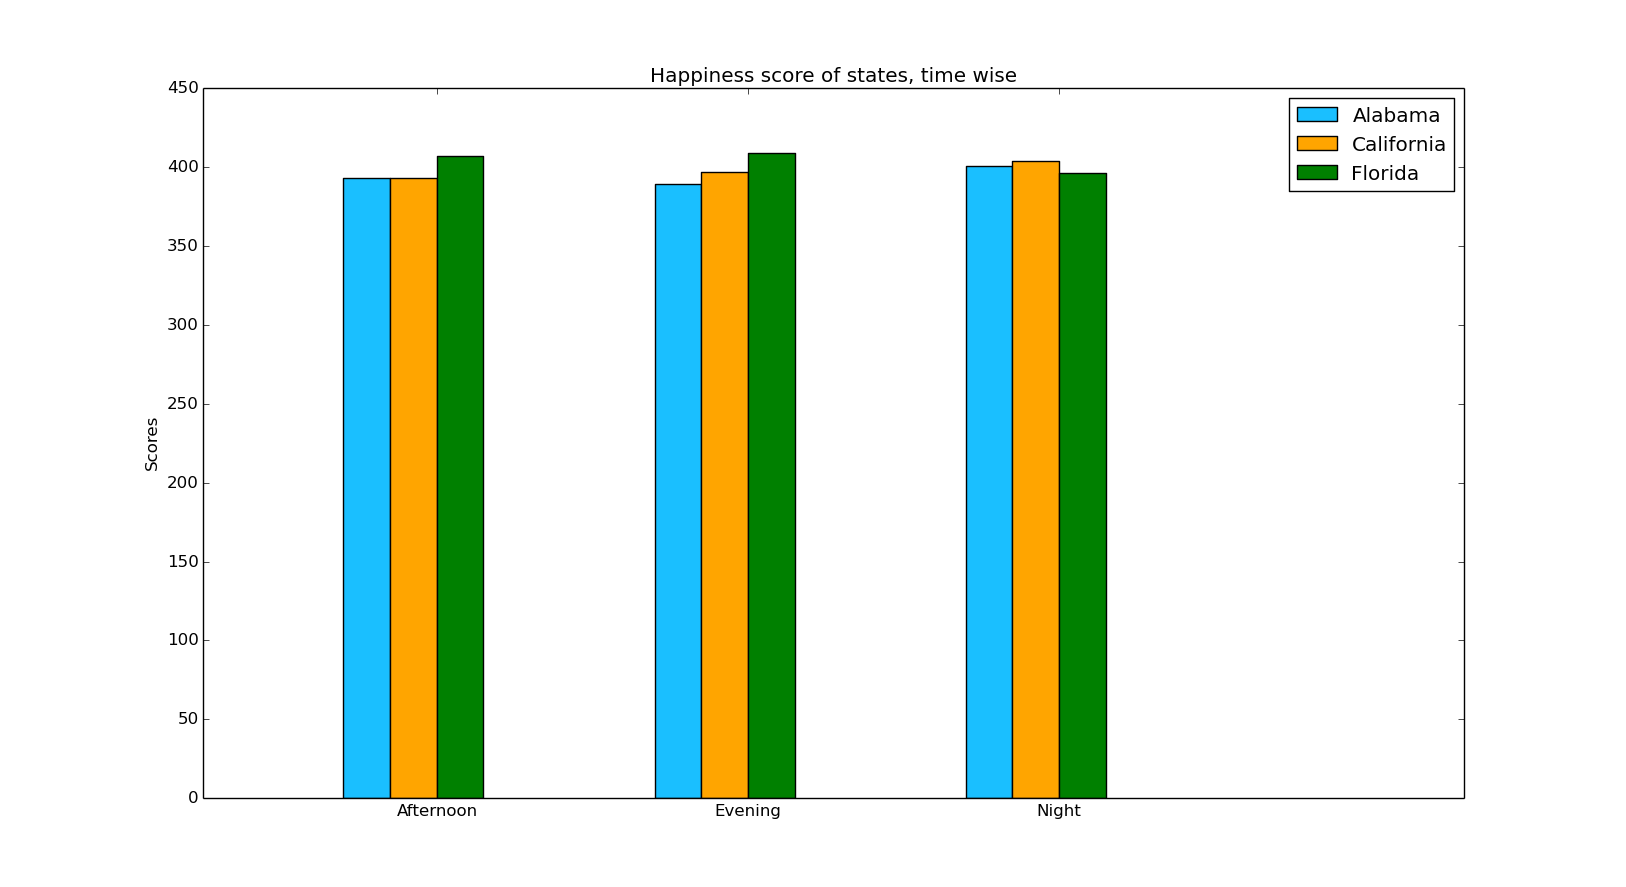
\includegraphics[scale=0.15]{./Images/Time_in_day500}
\caption{Happiness score for different times of the day for sample of 500 tweets}
\end{figure}
\end{columns}
\end{frame}

\subsection{Percentage}
\begin{frame}
\frametitle{Happiness score distribution contd.}
\begin{figure}
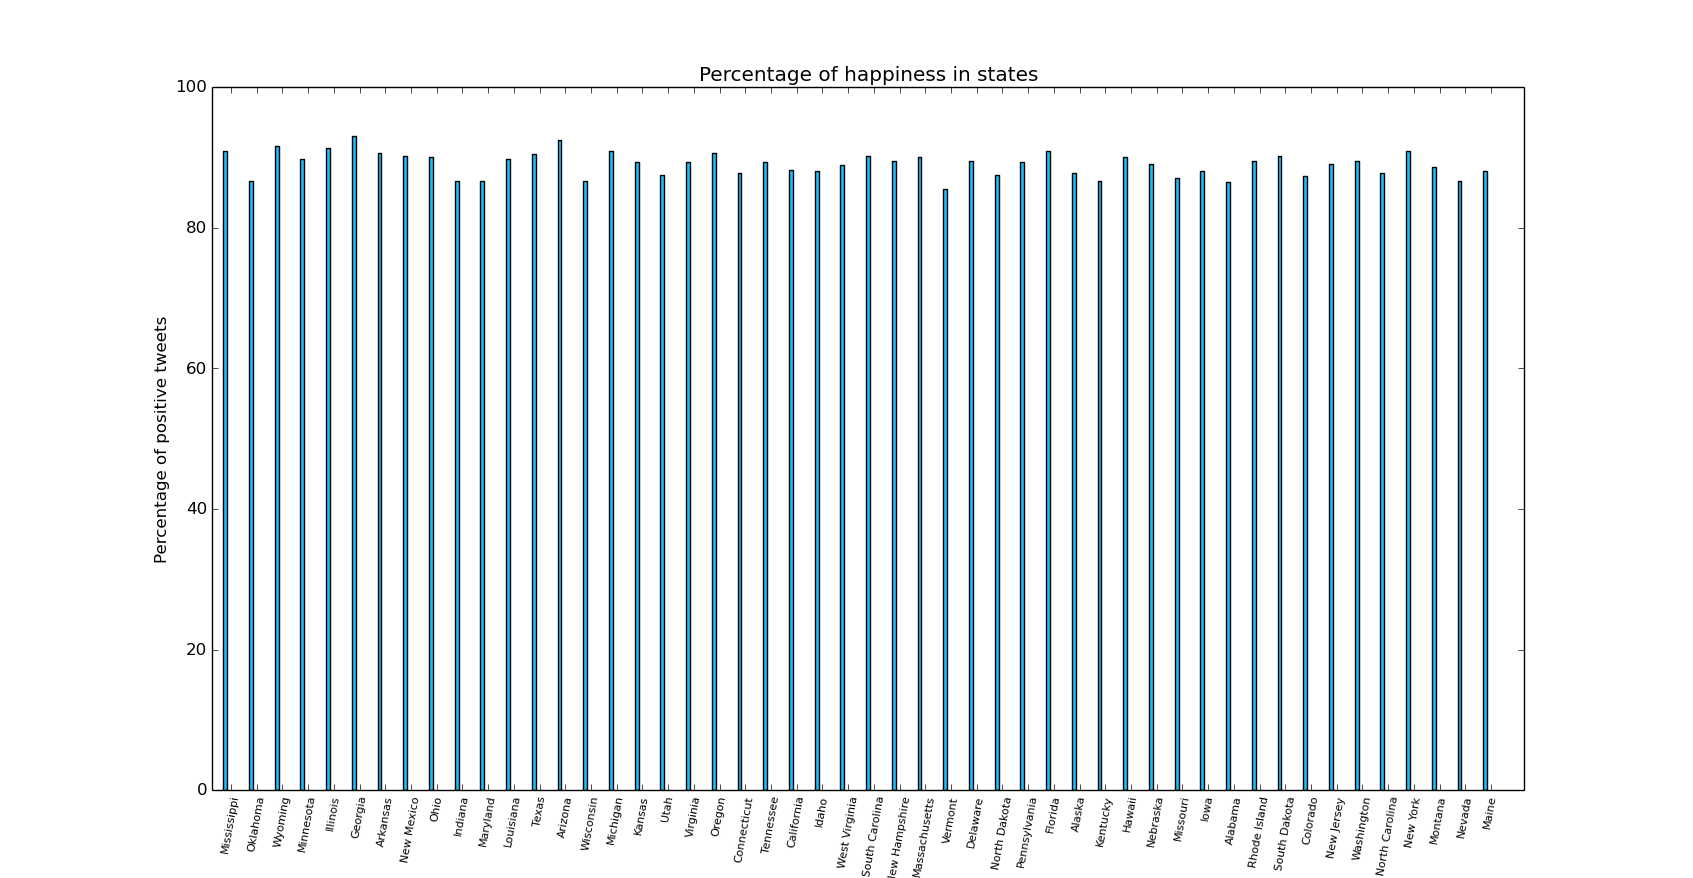
\includegraphics[scale=0.25]{./Images/Percentage}
\caption{Percentage of happiness in each state}
\end{figure}
\end{frame}

\subsection{State wise happiness distribution}
\begin{frame}
\frametitle{Happiness score distribution contd.}
\begin{figure}
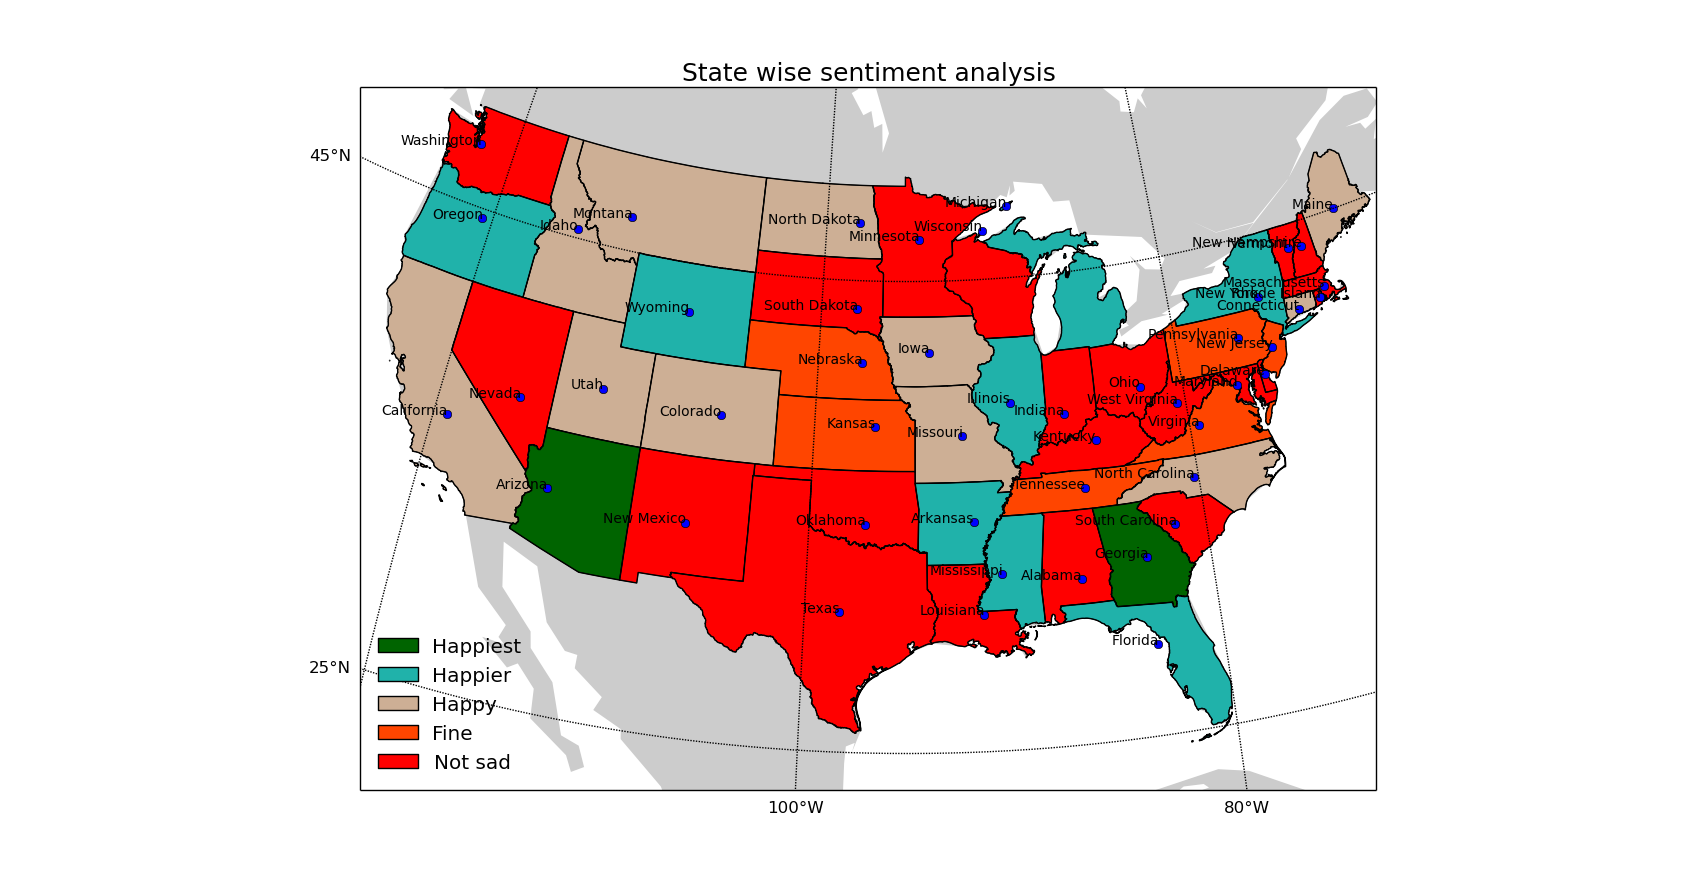
\includegraphics[scale=0.3]{./Images/GeoPlotFinal}
\caption{State wise geo-distribution of the happiness score}
\end{figure}
\end{frame}
\section{Conclusions}
\begin{frame}
\frametitle{Conclusions}
\begin{enumerate}
\item Happiest states are Arizona and Georgia
\item Almost all states are fairly positive since out of 500 tweets , minimum happy score is 320.
\item States with least scores are maximum.
\end{enumerate}
\end{frame}

\section{Bibliography}
\begin{frame}
\frametitle{Bibliography}
\begin{enumerate}
\item \url{https://dev.twitter.com/streaming/overview}
\item \url{http://www.laurentluce.com/posts}
\item \url{https://www.census.gov/geo/maps-data/data/cbf/cbf_state.html}
\item \url{http://stackoverflow.com}
\item \url{http://www.pythoncentral.io/introduction-to-tweepy-twitter-for-python}
\item \url{https://class.coursera.org/datasci-001/lecture/55}
\item \url{http://matplotlib.org/basemap/}
\end{enumerate}
\end{frame}
\end{document}
